

%%%%%%%%%%%%%%%%%%%%%%%%%%%%%%%%%%%%%%%%%%%%%%%%%%%%%%%%%%%%%%%%%%%%%%%%%%%%%%%%%%%%%
\section{Using Existing EMF Projects in eMoflon}
\label{sec : Ecore2GenModel}

Reuse of existing software components is common practice. Consider, for example, a well-tested software component you want to integrate in your current eMoflon project.
	
This chapter contains stepwise instructions how to use an existing EMF project within your eMoflon project. We exemplify this procedure by means of an \texttt{Ecore -> GenModel} transformation. The GenModel is an immediate representation of the Ecore models that contains additionally low level aspects for java code generation.

To the basic workflow for using an existing EMF-project in eMoflon is as follows:  First, the parts of the existing EMF-project you want to use in your own project have to be recreated in EA  (Section~\ref{sec: Set Up the Example}); Therafter, eMoflon has to be configured such that it does not generates code the reused project (as there still exists an implementation) but instead generates code for your project that it uses the code of existing project (Section~\ref{sec:Project Combination}).  




% This chapter is structured as follows:
% In Section~\ref{sec: Set Up the Example} the necessary projects for the example are set up. Section~\ref{sec:Project Combination} shows the actions required to use an existing project within an eMoflon project. 

\subsection{Set Up the Example} %  ---  SECTION  ---
\label{sec: Set Up the Example}

First, we have to set up the necessary projects, i.e., model the relevant parts \texttt{GenModel} in EA and implement the \texttt{Ecore -> GenModel} transformation. 

To model the relevant parts in EA:
\begin{enumerate}
\item[$\blacktriangleright$]Generate a new Moflon-Project \texttt{EcoreToGenModel} in Eclipse and switch to EA by doubel-clicking \texttt{EcoreToGenModel.eap}.

\item[$\blacktriangleright$]In EA, create the new \texttt{<<}EPackages\texttt{>>} \texttt{GenModel}.

\item[$\blacktriangleright$]Model part of GenModel as shows in Fig.~\ref{fig_gMM}.
\end{enumerate}
\begin{figure}[htbp]
\begin{center}  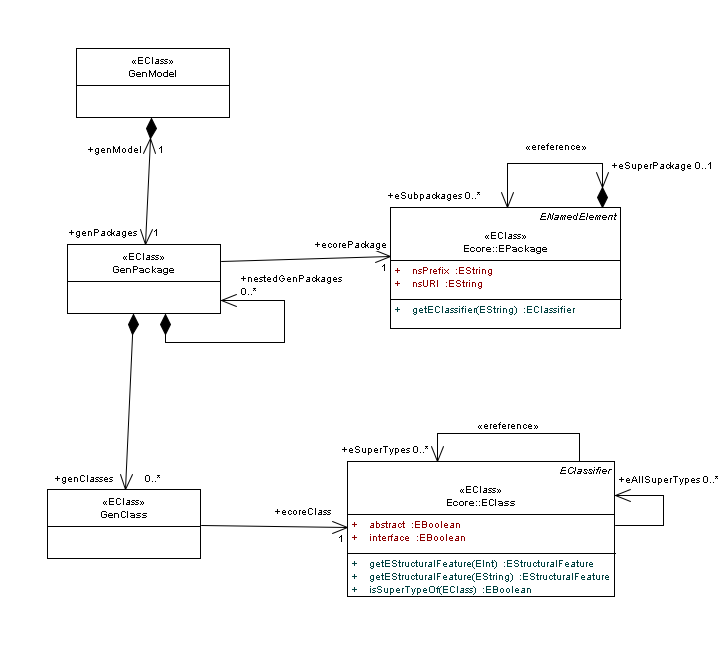
\includegraphics[width=1.0\textwidth]{pics/Ecore2GenModel_Bilder/EA_genMETAmodel.png}
        \caption{MetaModel of GenModel}  
  \label{fig_gMM}
\end{center}
\end{figure} 



The transformation should be located in the \texttt{Transformer} class shown in Figure~\ref{fig_e2gm}. 
\begin{enumerate}
\item[$\blacktriangleright$]In EA, create a new \texttt{<<}EPackages\texttt{>>} \texttt{Ecore2GenModel}.

\item[$\blacktriangleright$]Create the \texttt{Transformer} class as shown in Fig.~\ref{fig_e2gm}.
\end{enumerate}


The \texttt{Transformer} class has an operation to transform an \texttt{EPackage} to an \texttt{GenModel} (\texttt{epackageToGenModel(EPackage)}) and an operation to transform all \texttt{EPackages} to \texttt{GenPackages} (\texttt{transformEPackageToGenPackage(EPackage)}). The corresponding SDMs are shown in Figs.~\ref{fig_e2gm} and \ref{fig_transf}.

\begin{enumerate}
\item[$\blacktriangleright$] Implement the SDMs as shown by Figs.~\ref{fig_e2gm} and \ref{fig_transf}.
\end{enumerate}

% Next, we have to build a model where the actual transformation process is done.
% As you should be an expert on SDMs by now, we won't explain the SDMs in detail, here. Also, this is only one possibility of implementation.
% 
% When you look at the metamodel of GenModel ( Fig.~\ref{fig_e2gm}) you see that \texttt{Ecore} is a part of \texttt{GenModel}. A \texttt{GenClass} consists of \texttt{EClasses} and \texttt{GenPackage} consists of \texttt{EPackages}.
% Now, all we have to do is wrap \texttt{GenModel} around \texttt{Ecore} in the right order.
% 
% Fig.~\ref{fig_e2gm} shows the functions we choose for our implementation. We decided to do this as a recursive structure because an \texttt{EPackage} may consist of an undefined number of \texttt{eSubPackages}. To handle this the function \texttt{transformEPackageToGenPackage(EPackage)} performs a depth-first search for all nested sub-packages. Take a look at this function in Fig.~\ref{fig_transf}. The first StoryNode creates a new \texttt{GenPackage} and adds the bound \texttt{EPackage}. The next StoryNode \texttt{genClassesOfOnePackage} wrappes \texttt{GenClasses} around any \texttt{EClass} and puts them in the \texttt{GenPackage}. The other StoryNodes are for the recursive call.

\begin{figure}[htbp]
\begin{center}  
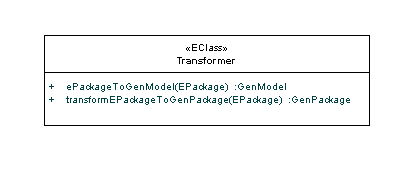
\includegraphics[width=0.8\textwidth]{pics/Ecore2GenModel_Bilder/EA_ecore2gM.png}
\caption{Transformer functions}  
\label{fig_e2gm}
\end{center}
\end{figure} 

\begin{figure}[htbp]
\begin{center}  
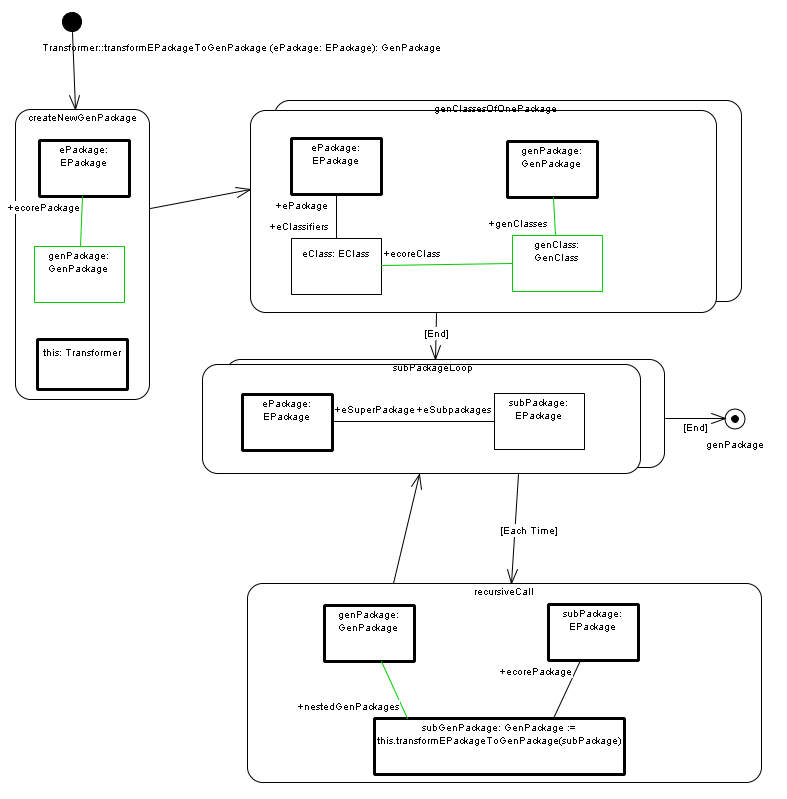
\includegraphics[width=1.0\textwidth]{pics/Ecore2GenModel_Bilder/EA_transPack2gM.png}
\caption{recursive function EPackage To GenPackage}  
\label{fig_transf}
\end{center}
\end{figure} 

% Since we want to have a \texttt{GenModel} and not only a \texttt{GenPackage} we need another function. The function \texttt{ePackageToGenModel(EPackage)} ( Fig.~\ref{fig_pack2gm}) takes a \texttt{EPackage} as parameter and checks if this \texttt{EPackage} is not nested in another \texttt{EPackage} itself. If this is the case \texttt{transformEPackageToGenPackage(EPackage)} will be called and the returned \texttt{GenPackage} will be included in the \texttt{GenModel}.

\begin{figure}[htbp]
\begin{center}  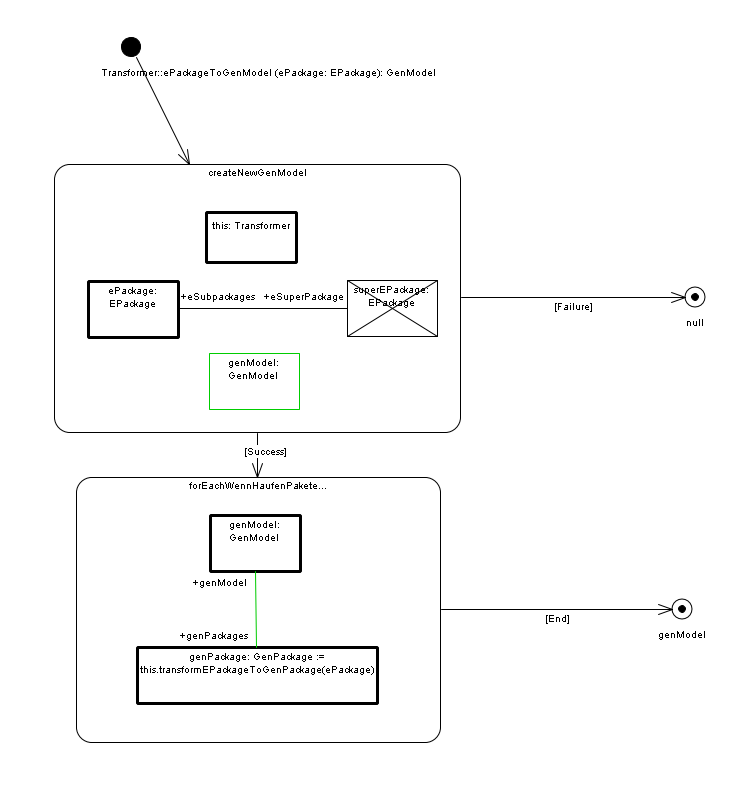
\includegraphics[width=1.0\textwidth]{pics/Ecore2GenModel_Bilder/EA_ePack2gM.png}
        \caption{EPackage To GenModel}  
  \label{fig_pack2gm}
\end{center}
\end{figure} 
  

\subsection{Project Combination} %  ---  SECTION  ---
\label{sec:Project Combination}

To integrate an eMoflon project into another one some parameters have to be set in eclipse and EA.

As the original code for GenModel still exists we don not need to export our replicated \textsf{GenModel}. To prevent eMoflon from generating code for a package:
\begin{enumerate}
\item[$\blacktriangleright$] Right-click the \texttt{<<}EPackage\texttt{>>} \textsf{GenModel}. Go to Properties/Moflon and change \texttt{Moflon::Export} to \texttt{false}.(Fig.~\ref{fig_customNS}).
\end{enumerate}

For correct code generation we have to tell EMF the real ``name'' of the project to be reused. To this end we tell eMoflon the correct \texttt{CustomNsPrefix} and \texttt{CustomNsUri}. To this end:
\begin{enumerate}
\item[$\blacktriangleright$] Create the tags  \texttt{Moflon::CustomNsPrefix} and \texttt{Moflon::CustomNsUri} for the \texttt{<<}EPackage\texttt{>>} \textsf{GenModel} and set them according to Fig.~\ref{fig_customNS}.
You can find these parameters by double clicking on the corresponding package in \texttt{.ecore} file.
\end{enumerate}

\begin{figure}[htbp]
\begin{center}  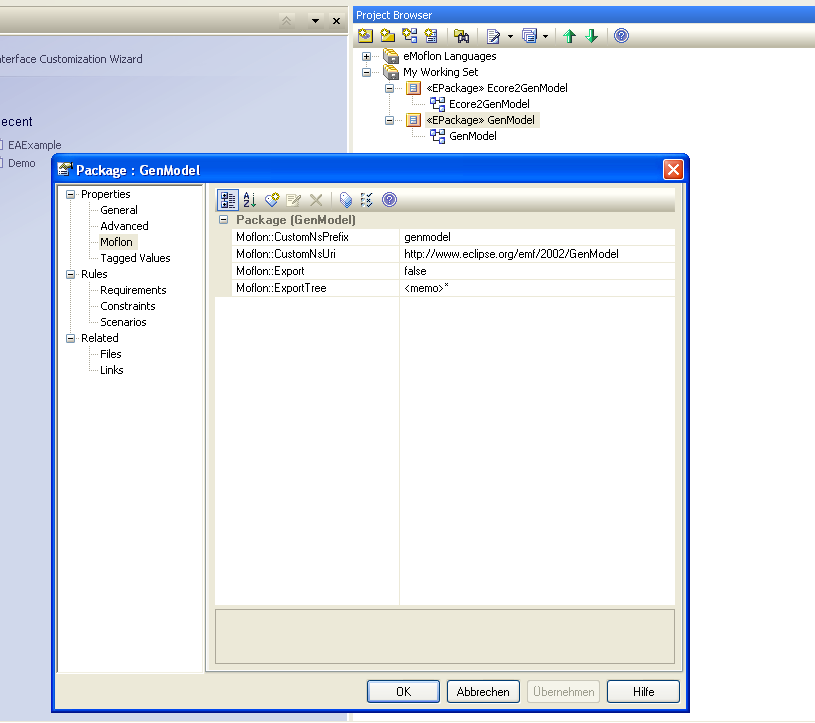
\includegraphics[width=0.7\textwidth]{pics/Ecore2GenModel_Bilder/8_nsUriPre.png}
  \caption{}  
  \label{fig_customNS}
\end{center}
\end{figure}

Now, we have set some properties in eclipse:

\begin{enumerate}
\item[$\blacktriangleright$]Export all to workspace. Switch back to eclipse and update the project with F5.

\item[$\blacktriangleright$]Change the eclipse project to a plug-in Tool. To do so, right-click the project \texttt{Ecore2GenModel} and then \texttt{Configure/Convert to Plug-in Projects...}.
We do this to make it easier to set the dependencies to the required EMF plugins. Otherwise each package in the plugin would have to be added separately.

\item[$\blacktriangleright$]To set the dependencies right-click \texttt{Ecore2GenModel} and then \texttt{Plug-in Tools/Open Manifest}.\\
In the window just opened click on the tab \texttt{Dependencies}. Then \texttt{Add} $org.eclipse.emf.codegen.ecore$. (This includes both the $Ecore$ and $GenModel$ libraries).


\end{enumerate}

Up to now, we told eMoflon the correct name (URI) of the project to be reused. Now we have to tell eMoflon where to find the existing project. 
\begin{enumerate}
\item[$\blacktriangleright$]Open the \texttt{moflon.properties} file located in your project folder; create the  properties \\ \texttt{ADDITIONAL\_DEPENDENCIES} and \texttt{ADDITIONAL\_USED\_GEN\_PACKAGES} and  set them to the path of the \texttt{.ecore} and \texttt{.genmodel} file of the reused project, respectively. For the example insert the following lines:
\begin{enumerate}
  \item[$\blacktriangleright$] \texttt{{\tiny ADDITIONAL\_DEPENDENCIES=platform:/plugin/org.eclipse.emf.codegen.ecore/model/GenModel.ecore}}
  \item[$\blacktriangleright$] \texttt{{\tiny ADDITIONAL\_USED\_GEN\_PACKAGES=platform:/plugin/org.eclipse.emf.codegen.ecore/model/GenModel.genmodel}}
\end{enumerate}
\end{enumerate}


In case you have chosen a name for the replicated package that differs from the real-one you have to define a name mapping to correctly resolve the imports.

\begin{enumerate}
	\item[$\blacktriangleright$] The import mapping property looks the following :
	\begin{enumerate}
		\item [$\blacktriangleright$]\texttt{IMPORT\_MAPPINGs=`your name' -> `real name'}. 
	\end{enumerate}
	\item [$\blacktriangleright$]Regarding the example insert the following line:
	\begin{enumerate}
  		\item [$\blacktriangleright$]\texttt{\footnotesize IMPORT\_MAPPINGS=genmodel-> org.eclipse.emf.codegen.ecore.genmodel}
	\end{enumerate}
\end{enumerate}


\begin{enumerate}
		\item [$\blacktriangleright$]TODO missing FactoryMapping
	\end{enumerate}

Now the moflon.properties file should look as depicted in Fig.~\ref{fig_mofProp}

\begin{figure}[htbp]
\begin{center}  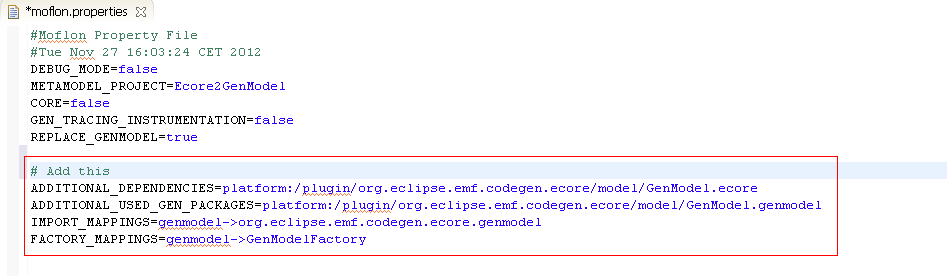
\includegraphics[width=1.3\textwidth]{pics/Ecore2GenModel_Bilder/9_mofProperties.png}
  \caption{}  
  \label{fig_mofProp}
\end{center}
\end{figure}  







